\documentclass[parskip=full]{uvamscse}

\setcounter{secnumdepth}{4}

\titleformat{\paragraph}
{\normalfont\normalsize\bfseries}{\theparagraph}{1em}{}
\titlespacing*{\paragraph}
{0pt}{3.25ex plus 1ex minus .2ex}{1.5ex plus .2ex}

\usepackage{listings}

\lstdefinelanguage{sdf}{%
  numbers=none,
  morekeywords={module,imports,exports,sorts,context,lexical,free,syntax,==,=,+,-,left,cons,prefer,avoid,bracket},
  columns=flexible,
  morestring=[b]",
  basicstyle=\footnotesize\mdseries,
  literate={->}{{\,\,$\to$\,\,}}1
}

\lstdefinelanguage{dcg}{%
  numbers=none,
  morekeywords={},
  morestring=[b]",
  basicstyle=\footnotesize\mdseries,
  columns=flexible,
}

\lstdefinelanguage{prolog},
  literate={:-}{{\,$\Leftarrow$\,\,}}1 {-->}{{$\to$\,}}1
}

\lstdefinestyle{mono}{
  basicstyle=\footnotesize\ttfamily
}

\lstset{%
  frame=none,
  xleftmargin=2pt,
  stepnumber=1,
  numbers=left,
  numbersep=7pt,
  numberstyle=\ttfamily\scriptsize\color[gray]{0.3},
  belowcaptionskip=\bigskipamount,
  captionpos=b,
%  escapeinside={*'}{'*},
  % language=fl,
  tabsize=2,
  emphstyle={\bf},
  stringstyle=\itshape,
  showspaces=false,
  keywordstyle=\bfseries\rmfamily,
  columns=flexible,
  basicstyle=\small\mdseries,
  showstringspaces=false,
}

\newcommand{\cmd}[1]{\texttt{$\backslash$#1}}

\title{Detecting Violations of CSS Code Conventions}
% \coverpic[100pt]{figures/terminal.png}
% \subtitle{}
% \date{Spring 2014}


\author{Boryana Goncharenko}
\authemail{boryana.goncharenko@gmail.com}
% \host{Grammarware, Inc., \url{http://grammarware.github.io}}

\abstract{    

Code conventions are used to preserve code base consistency and express preference of a particular
programming style. Often, code conventions are expressed in natural language and it is a
responsibility of the developers to read, understand and apply them. Typically, developers need to
ensure that their code complies to a given style guide manually. There are a number of tools that
can automatically detect violations of conventions, however, current solutions remain rigid,
laborious or with limited scope.

This thesis aims at answering three research questions. First, it evaluates the need for CSS
conventions based on whether CSS is still handcrafted. Second, it discovers existing code
conventions. Third, it designs a domain-specific language that is capable of expressing existing CSS
code conventions. The thesis presents a specification of the designed domain-specific language and an implementation of its interpreter that detects violations automatically.

}


\begin{document}
\maketitle

%%%%%%%%%%%%%%%%%%%%%%%%%%%%%%%%%%%%%%%%%%%%%%%%%%%%%%%%%%%%%%%%%%%%%%%%%%%%%%%%
\chapter{Introduction}

Code conventions put constraints on how code should be written in the context of a project,
organization or programming language. Style guides can comprise conventions that refer to
whitespacing, indentation, code layout, preference of syntactic structures, code patterns and anti-
patterns. They are mainly used to achieve code consistency, which in turn improves the readability,
understandability and maintainability of the code~\cite{Buse2010} ~\cite{buse2010learning}
~\cite{tenny1988program}.

Style guides are often designed in an ad hoc manner. Coding conventions typically live in documents
that contain a description of each rule in natural language accompanied by code examples. This is
the case with the style guidelines of Mozilla~\cite{Mozilla}, Google~\cite{Google},
GitHub~\cite{GitHub}, WordPress~\cite{Wordpress} and Drupal~\cite{Drupal}. It is the responsibility
of the developers to ensure that their code complies to a given style guide. Typically, they need to
read and understand the conventions and then apply them manually. Such an approach introduces a
number of issues. First, using natural language can make guidelines incorrect, ambiguous, implicit
or too general. Second, the fact that developers apply conventions manually increases the chances of
introducing violations involuntarily. There are a number of tools that can automatically detect
violations of conventions, however, current solutions are often hard to customize or are limited to
one type of violations, e.g. only whitespacing.

The core idea behind the project is to provide a solution that lets developers express an arbitrary
set of coding conventions and detect their violations automatically. Writing conventions
in an executable form could assist authors in detecting incorrect, ambiguous or inconsistent
guidelines. Automatic detection of violations could minimize the effort required by developers to
write code that complies to the guidelines. To meet the constraints of a Master’s project, the
implementation is limited to the domain of Cascading Style Sheets (CSS). The project requires
determining the need for CSS code conventions in organizations, collecting and analyzing available
style guides, and providing a way to express conventions. Specifically, the project attempts to
answer the following set of questions:

  \begin{description}
    \item \textbf{Research Question 1} Do developers still maintain plain CSS?
    \item \textbf{Research Question 2} What code conventions for CSS exist?
    \item \textbf{Research Question 3} How to express existing CSS code conventions?
  \end{description}

The thesis is organized as follows. Chapter \ref{sec:background} provides information about previous
studies and defines concepts and terms used throughout the thesis. Chapter \ref{sec:evaluating}
presents the research approach used to determine whether CSS is handcrafted and analysis of the
gathered results. Chapter \ref{sec:discovering} contains the research method  used to discover
existing code conventions and the results of the research. The design and validation of the DSL are
presented in Chapter \ref{sec:expressing}. Chapter \ref{sec:conclusion} concludes the thesis.


%%%%%%%%%%%%%%%%%%%%%%%%%%%%%%%%%%%%%%%%%%%%%%%%%%%%%%%%%%%%%%%%%%%%%%%%%%%%%%%
\chapter{Background}
\label{sec:background}

\section{Bunge-Wand-Weber ontology}

A \textbf{conceptualization} is an abstract, simplified view of the world that is represented for
some purpose~\cite{gruber1995toward}. It consists of the concepts that are assumed to exist in some
area of interest and their relationships~\cite{gruber1995toward}. An \textbf{ontology} is an
explicit specification of a conceptualization~\cite{gruber1995toward}. It describes what is
fundamental in the totality of what exists and it defines the most general categories to which we
need to refer in constructing a description of reality~\cite{milton2004top}.

Researchers distinguish between two kinds of ontologies: top-level and domain-
specific~\cite{milton2004top}. Ontologies of the former type are highly general and provide the
theoretical foundations for representation and modeling of systems. Ontologies of the latter type
define concepts and their relations only for a particular domain. A domain- specific ontology is
based on a specific top-level ontology if it uses the categories defined by the high level
ontology~\cite{milton2004top}.

The Bunge-Wand-Weber (BWW) ontology~\cite{wand1990ontological} is a high-level ontology used in the
representation model developed by Wand and Weber~\cite{wand1995deep}. Table \ref{tab:bwwmodel}
presents a selected set of the ontological constructs in the BWW ontology.

\begin{center}
\begin{longtable}{ | p{11em} | p{30em} | } 
\caption{Selected ontological constructs in the BWW representation model}
\label{tab:bwwmodel}\\
\hline
 &  \\
\textbf{Ontological construct} & \textbf{Explanation} \\
 &  \\
\hline
Thing & The elementary unit in the BWW ontological model. The real world is made up of things. A composite thing may be made up of other things (composite or primitive).~\cite{wand1995deep} \\ 
\hline
Properties & \multirow{7}{30em}{Things possess properties. A property is modeled via a function that maps the thing into some value. A property of a composite thing that belongs to a component thing is called an hereditary property. Otherwise it is called an emergent property. A property that is inherently a property of an individual thing is called an intrinsic property. A property that is meaningful only in the context of two or mode things is called a mutual or relational property.~\cite{wand1995deep}} \\ 
 &  \\ 
 &  \\
 &  \\
 &  \\
 &  \\
 &  \\
 \hline
 State & A vector of values for all property functions of a thing.~\cite{wand1995deep} \\
 \hline
 Event & A change of state of a thing. It is effected via a transformation.~\cite{wand1995deep} \\
 \hline
 Transformation & A mapping from a domain comprising states to a codomain comprising states.~\cite{wand1995deep} \\
 \hline
 History & The chronologically ordered states that a thing traverses.~\cite{weber1996analytical} \\
 \hline
 Coupling & A thing acts on another thing if its existence affects the history of the other thing. The two things are said to be coupled or interact.~\cite{wand1995deep} \\
 \hline
 Class & A class is a set of things that can be defined via their possessing a characteristic property.~\cite{weber1996analytical} \\ 
 \hline
 Subclass & A set of things that can be defined via their possessing the set of properties in
a class plus an additional set of properties.~\cite{weber1996analytical} \\ 
\hline
 System & A set of things is a system if, for any bi-partitioning of the set, couplings exist among things in the two subsets.~\cite{wand1995deep} \\
 \hline
 System Composition & The things in the system are its composition.~\cite{wand1995deep} \\
 \hline
 System Environment &  Things that are not in the system but interact with things in the system are called the environment of the system.~\cite{wand1995deep} \\
 \hline
\end{longtable}
\end{center}


\section{Ontological analysis}

\textbf{Ontological analysis} is an established approach for evaluating the quality of software engineering notations~\cite{moody2009physics}. It consists of a two way comparison between a set of modeling grammar constructs and a set of ontological constructs. The \textbf{interpretation mapping} compares the notation with the ontology and the \textbf{representation mapping} compares the ontology with the notation~\cite{gehlert2007toward}. The underpinning of ontological analysis is that modeling grammars are incomplete if they are not able to represent what exists in reality~\cite{green2000integrated}. Furthermore, the analysis requires one-to-one mapping between the modeling grammar and the ontological constructs. Any deviation from such correspondence leads to a discrepancy (Figure \ref{fig:ontoanalysis}).

\begin{figure}[h!]
  \centering
  \caption{Ontological Analysis~\cite{gehlert2007toward}}
  \label{fig:ontoanalysis}
  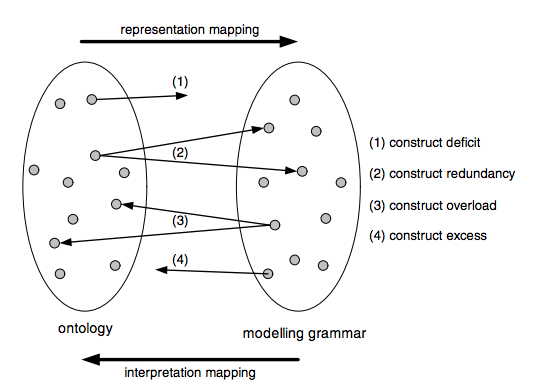
\includegraphics[width=0.65\textwidth]{ontoanalysis}
\end{figure}

\textbf{Construct deficit} occurs when an ontological construct does not have a corresponding construct in the modeling grammar. \textbf{Construct redundancy} is observed when a single ontological construct maps to more than one modeling grammar construct. \textbf{Construct overload} appears when a modeling grammar construct corresponds to more than one ontological construct. \textbf{Construct excess} emerges when a modeling grammar construct does not map to any ontological construct.~\cite{moody2009physics}

%%%%%%%%%%%%%%%%%%%%%%%%%%%%%%%%%%%%%%%%%%%%%%%%%%%%%%%%%%%%%%%%%%%%%%%%%%%%%%%
\chapter{Evaluating the Need for CSS Code Conventions}
\label{sec:evaluating}

\section{Research Method}

Despite the new features added in the second~\cite{CSS2} and third~\cite{CSS3} versions of CSS, the
language has obvious limitations, for example, lack of variables. A number of preprocessors have
evolved to tackle the downsides of CSS. Solutions such as SASS~\cite{SASS}, LESS~\cite{LESS} and
Stylus~\cite{Stylus} offer enhanced or even different syntax and translate it to CSS. Preprocessors
are not only ubiquitously recommended, but also widely adopted in practice. The presence of such
solutions poses the question whether conventions for CSS are required at all. If nowadays CSS is
generated and not maintained, the need for CSS conventions is substituted with need for preprocessor conventions.

To determine whether CSS is still handcrafted, all commits to open source repositories hosted on
GitHub for the period Jan-Apr 2015 were analyzed. To differentiate between plain CSS and
preprocessor code, the extensions of all files in the commits were inspected. In case the commit
contains a file with extension \texttt{.scss}, \texttt{.sass}, \texttt{.less} or \texttt{.styl}, it
is considered preprocessor maintenance. In case the commit contains files with the \texttt{.css}
extension and no preprocessor extensions, it is considered maintenance of plain CSS. Since the main
objective of the search is finding maintained files, only files that have been modified are taken
into consideration. Files that have been added are excluded from the results, since developers often
add third-party CSS libraries to their repositories.


\section{Results}

A total of 1,589,713 commits to 1,311,654 public repositories have been analyzed. X of these were
not processed due to errors. Typical errors contain repositories that have been turned private
and... The number of commits that maintain any form of CSS is X. Figure \ref{cssresults} summarizes
the findings.

\begin{figure}[h!]
  \centering
  \caption{Results}
  \label{cssresults}
  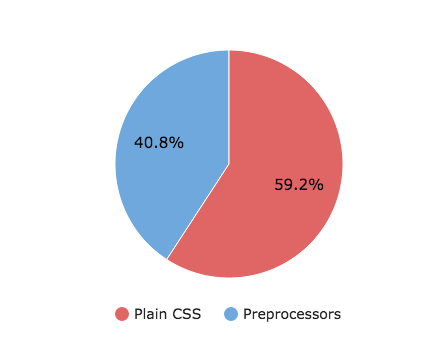
\includegraphics[width=0.5\textwidth]{cssresults}
\end{figure}

\section{Analysis}

There are a number of limitations that need to be considered before interpreting the results of the
conducted research. Firstly, the search is conducted on a single hosting platform - GitHub. That
said, currently GitHub reports having over 10 million users and 24 million
repositories~\cite{GitHub}, which makes it the largest code host in the
world~\cite{gousios2014lean}. Secondly, the search is narrowed to the publicly available
repositories. Thus, it lies on the premise that there is not a significant difference between the
public and private repositories hosted on the platform. Thirdly, the search detects only the four
most popular preprocessor extensions and omits other preprocessors. It is possible that a number of
custom preprocessors are used in practice. However, it is assumed that the number of such commits
would not increase the number of total CSS commits to the extend at which the percentage of plain
CSS commits is significantly diminished.

Having the above limitations in mind, the search provides evidence to conclude that despite the
popularity of preprocessors, plain CSS is still handcrafted on GitHub in the beginning of 2015.

%%%%%%%%%%%%%%%%%%%%%%%%%%%%%%%%%%%%%%%%%%%%%%%%%%%%%%%%%%%%%%%%%%%%%%%%%%%%%%%

\chapter{Discovering Existing CSS Code Conventions}
\label{sec:discovering}

\section{Research Method}

The primary organization responsible for the specification of CSS has not published an official CSS
style guide. As a result, the CSS community has produced a pool of coding conventions, best
practices, guidelines and recommendations.

To discover existing CSS code conventions, two searches with the keywords \texttt{CSS code
conventions} were made using the search engines \url{http://duckduckgo.com} and
\url{http://google.com}. The first 100 results of each search were analyzed. From each result
only conventions that refer to plain CSS are taken into account and conventions related to
preprocessors are ignored. In case the result contains links to other style guides, these
references are considered as results and analyzed separately.

While searching for conventions, a number of issues were discovered. First, some of the
conventions do not provide sufficient information to be applied in practice. Such an example is the
convention \textit{Do not use CSS hacks - try a different approach first} when the style guide does
not define the meaning of CSS hacks. Such overgeneralized conventions were omitted from the results.

Another part of the discovered conventions introduce a discrepancy between their description in
natural language and the provided code example. An instance of such contradiction is when the
convention \textit{Nothing but declarations should be indented} is followed by a code snippet
illustrating that rules in media queries should also be indented. In such cases the convention is
interpreted as described by the code example.

When conventions are not supported with code examples, their description could remain open for
interpretation. For example, \textit{Rules with more than 4 selectors are not allowed} could be seen
as forbidding multi-selectors with more than four selectors, or disallowing selectors with more than
four simple-selectors. All possible interpretations of ambiguous conventions were registered as
separate conventions.

There are conventions that are not explicitly stated, but could only be inferred by the other rules.
For example, the convention \textit{You can put long values on multiple lines} states that a long
value is allowed to appear on several lines. However, this rule implies the presence of another
convention, that is not explicitly stated. It implies that short values should appear on one line
and only lengthy values are allowed to appear on multiple. Such implicit conventions were registered
as explicit conventions.

\section{Results}

As a result of the searches, a corpus of 165 unique CSS code conventions was accumulated. Sources
of these conventions include CSS professionals, open-source communities and companies, such as \href{https://google-styleguide.googlecode.com/svn/trunk/htmlcssguide.xml#Protocol}{Google}, \href{http://primercss.io/guidelines/#css}{GitHub}, \href{https://make.wordpress.org/core/handbook/best-practices/coding-standards/css/}{Wordpress}, \href{https://www.drupal.org/node/1887862}{Drupal}. The following list presents a selected set of the discovered conventions:

\begin{itemize} 
\item Avoid qualifying ID and class names with type selectors. 
\item Use RGBA only when opacity is needed.
\item Use short hexadecimal values. 
\item CSS files must not include any @charset statements.
\item Disallow @import. 
\item When possible, use em instead of pix. 
\item Avoid using z-indexes when possible. 
\item Require compatible vendor prefixes. 
\item Do not use !important. 
\item Do not use id selectors. 
\item Id and class names should be lowercase.
\item All values except the contents of strings should be lowercase.  
\item HTML tags should be lowercase.
\item Put a ; at the end of declarations. 
\item Do not put quotes in URL declarations.
\item Use short hex values.
\item Use the shorthand margin property.
\item Do not use units after 0 values.
\item Use a leading zero for decimal values.
\item Use single quotes in charsets.
\item Use single quotes in attribute selectors.
\item Put one space between the colon and the value of a declaration.
\item Put one space between the last selector and the block.
\item One selector per line.
\item A rule must not contain height and border, border-top, border-bottom, padding, padding-top, or padding-bottom.
\item A rule must not contain width and border, border-left, border-right, padding, padding-left, or padding-right.
\item Warning if a property is included in a rule twice and contains the same value.
\item Forbid empty rules.
\item A vendor-prefixed property must be followed by a standard property.
\item Require fallback color. A color property with a RGBA(), HSL(), or HSLA() color without a preceding color property that has an older color format.
\item A rule that has display: inline-block should not use float.
\item A rule that has display: block should not use vertical-align.
\item Use 4 spaces for indentation, no tabs.
\item No trailing spaces.
\end{itemize}

The full list of all discovered conventions along with their sources and explanation of their meaning is available in \href{https://github.com/boryanagoncharenko/CssCoco/blob/master/analysis.md}{CssCoco GitHub repository}.

%%%%%%%%%%%%%%%%%%%%%%%%%%%%%%%%%%%%%%%%%%%%%%%%%%%%%%%%%%%%%%%%%%%%%%%%%%%%%%%

\chapter{Expressing CSS Code Conventions}
\label{sec:expressing}

\section{Analysis of conventions corpus}

Code conventions is an umbrella term that comprises rules for whitespacing, comments, indentation,
naming, syntax, code patterns, programming style, file organization etc. To gain an overview of the
type of conventions used in the CSS domain, all conventions in the corpus are organized in groups
depending on the type of constraints they impose. The following three categories were defined
(sublists provide examples of conventions that fall in each category):

\begin{description}
  \item[Layout] category contains rules that constrain the overall layout of the code. It includes conventions related to whitespace, indentation and comments. Examples include:
  \begin{itemize}
  \item Use four tabs for indentation.
  \item Put one blank line between rulesets.
  \item Disallow spaces at the end of the line.
  \end{itemize}
  \item[Syntax Preference] category comprises conventions that express preference of a particular syntax. Note that rules in this category do not aim at ensuring CSS validity, but choose between syntactic alternatives. For example, both single and double quote strings are valid in CSS and a convention may narrow down the choice of the developer to single quotes. Examples include:
  \begin{itemize}
  \item Use lowercase for id and class names.
  \item Require a semicolon at the end of the last declaration.
  \item Use strings with single quotes.
  \end{itemize}
  \item[Programming Style] category consists of conventions that put constraints on how CSS constructs are used to achieve a certain goal. They specify preferred code patterns or anti-patterns. Conventions in this group are used mainly to improve maintenance and performance, or to avoid a bug in a particular implementation. Examples are:
  \begin{itemize}
  \item Do not use the universal selector.
  \item Avoid using !important.
  \item A vendor-prefixed property must be followed by a standard property.
  \end{itemize}
\end{description}

Conventions in each of the groups were analyzed and their violations were made explicit. While the
violations of most of the conventions are obvious, some of them require knowledge about the possible
valid CSS syntax. For example, conventions such as \textit{Avoid id selectors} directly describe
their violations - id selectors. That said, the convention \textit{Use single quotes in URLs} has
two violations: URLs with single quotes and URL without quotes.

After the violations of each convention were made explicit, the specific actions needed to detect
these violations were determined. Currently, the detection of violations is performed by developers
manually or with the partial help of tools. To perform such checks, developers need to understand
different concepts, e.g. the concept of a rule, HTML element, IDs, etc and perform certain actions,
such as find a structure, evaluate a constraint etc. The analysis tries to grasp the specific
concepts and actions used to find violations. To illustrate the process, the analysis of one convention is included. Analysis of all conventions in the corpus is available at
\href{https://github.com/boryanagoncharenko/CssCoco/blob/master/analysis.md}{CssCoco GitHub
repository}.

\begin{description}
\item\textbf{Convention:} Disallow empty rules.
\item\textbf{Author:} \href{https://github.com/CSSLint/csslint/wiki/Disallow-empty-rules}{CSS lint}
\item\textbf{Violations:} Presence of rulesets that do not contain declarations. In case at least one declaration is present, the ruleset does not violate the convention. Examples include:
\begin{sourcecode}
\begin{lstlisting}[style=mono,language=Java]
.myclass { }                 /* violation */
.myclass { /* Comment */ }   /* violation */
.myclass { color: green; }   /* not violation */
\end{lstlisting}
\end{sourcecode}

\item\textbf{Actions:} Recognize rulesets and declarations. Determine whether a ruleset does not contain any declarations.

\item\textbf{Analysis:} The convention aims at getting rid of one type of refactoring leftovers -
rulesets without declarations. Removing empty rulesets reduces the total size of CSS that
needs to be processed by the browser. One possible approach for discovering violations of the
convention at hand is to search the stylesheet for rulesets and then check whether each ruleset
contains a declaration. To perform this search successfully, developers need to understand the
concept of a ruleset and a declaration, i.e. they need to be able to recognize these two CSS
structures. Further, developers need to determine relations between structures, particularly,
whether a ruleset contains a declaration.

\end{description}


After all conventions were analyzed, the specific actions and concepts were used to extract
requirements and draw conclusions about the needed functionality. First, every convention can be
represented as a combination of constraints, regardless of the way it is expressed. There are two
major constructs used to convey conventions in natural language: forbid and require. Conventions
that forbid describe directly their violations. For example, the convention \textit{Disallow
@import} specifies that import statements are violations. Conventions that use the latter construct
describe a pattern and once the pattern is found the constraint is evaluated. In case the constraint
is not met, a violation is discovered. For example, the convention \textit{class names should be
lowercase} requires finding class nodes and then checking whether they are lowercase.

As the three categories of conventions imply, conventions can reference nodes from the abstract
syntax tree, concrete syntax tree and parse tree of CSS. For example, the convention \textit{A rule
must not contain width and padding declarations} accesses concepts that are present in the abstract
syntax tree. Similarly, the rule \textit{Put a semicolon at the end of the last declaration} refers
to nodes that are omitted by the abstract syntax tree and are present in the concrete syntax tree.
All whitespacing and indentation conventions target nodes that are relevant only in the parse tree
of CSS.

Conventions refer to nodes using their type or function in the CSS program. For example, in the
snippet \texttt{[class=``test'']} the node test can be selected 1) because it is of type string and
2) because it is an attribute value. Similarly, a node with value \texttt{\#ffffff} may be selected
because it is a hexadecimal value or because it represents a color.

Conventions may use CSS-specific knowledge. For example, the rule \textit{Use lowercase for
properties; vendor-prefixed properties are exception} requires differentiating between standard and
vendor-specific properties. While in this case the two types of properties can be easily
distinguished, some conventions require information that cannot be obtained using the CSS code.
Consider the convention \textit{Order vendor-prefixed values by their version; newer versions of
vendor values should appear after old ones}. To detect violations for this convention the release
dates of the properties need to be available for comparison.

Conventions rarely target a single node. Typically, they refer to a number of nodes organized in a
pattern. For example, the convention \textit{A ruleset must not contain display and float
declarations} requires searching for two specific declaration that appear under the same parent
node. The nodes in the pattern do not have to be immediate relatives. In fact, they can be scattered
across the tree. For example, the rule \textit{Do not use more than 5 @font-face declarations}
requires searching for specific nodes that appear anywhere in the tree.

\section{CssCoco DSL}

\subsection{Syntax overview}

To express the conventions in the corpus, the domain-specific language CssCoco is proposed. It is a
declarative language that has two main constructs: conventions and contexts. Conventions express the
specific rules that has to be enforced on the code and contexts describe the CSS nodes that need to
be ignored while searching for violations. 

The language constructs that define conventions try to resemble the way conventions are expressed in
natural text. There is a construct that describes directly what is disallowed. For example, the
convention \textit{Do not use import statements} is expressed in the following way:

\begin{sourcecode}
\begin{lstlisting}[style=mono,language=Java]
forbid import
message 'Do not use import statements.'
\end{lstlisting}
\end{sourcecode}

The keyword \textit{forbid} is followed by a description of the node that is disallowed. In the
current convention, we only need to state its type - import. Each convention requires a message
clause. The string after the \textit{message} keyword will be displayed to the user, when a
violation is found.

As domain analysis indicates, conventions are often expressed as a pattern that, if found, needs to
meet given constraints. In CssCoco syntax such conventions are defined using the \texttt{find ...
require ...} construct. For example, the convention \textit{All class names should be lowercase} is
described as follows:

\begin{sourcecode}
\begin{lstlisting}[style=mono,language=Java]
find c=class
require c.name match lowercase
message 'All id and class names should be lowercase'
\end{lstlisting}
\end{sourcecode}

The find clause in the above rule specifies the pattern that needs to be found and the require
clause states the constraint that should be applied to the discovered nodes. Note that to refer to a
matched node in the require clause, the node should be assigned as identifier, \texttt{c} in the
above example.

Conventions can put more constraints on a node description in the pattern. For example, the
convention \textit{Use a leading zero for decimal values} requires finding all nodes of type number
that have a numeric value in the interval [-1, 1]. Such constraints are expressed as curly brackets
immediately after the type of the node.

\begin{sourcecode}
\begin{lstlisting}[style=mono,language=Java]
find n=number{num-value < 1 and num-value > -1}
require n.string match '^0.*'
message 'Use a leading zero for decimal values'
\end{lstlisting}
\end{sourcecode}

Conventions can describe patterns that consist of more than one node. For example, the rule
\textit{Use single quotes in charsets} can be expressed in the following way:

\begin{sourcecode}
\begin{lstlisting}[style=mono,language=Java]
find s=string in charset
require s.has-single-quotes
message 'Use single quotes in charsets'
\end{lstlisting}
\end{sourcecode}

The pattern contains the description of two nodes: first, a node that is of type string and a node
of type charset. The \texttt{in} keyword description of the pattern indicates that the string node
is nested in the charset node. In this way, the pattern will match only the strings that appear in a
charset.

In CssCoco conventions are grouped in contexts that specify what nodes should be ignored when
searching for patterns. For example, often when rules refer to newlines they completely disregard
indentation. The convention \textit{Every declaration must be on a new line} requires a newline to
be present immediately before the declaration. However, when declarations are indented their
immediate previous sibling is an indentation node. To handle such cases, the language uses contexts
that explicitly describe the ignored nodes.

\begin{sourcecode}
\begin{lstlisting}[style=mono,language=Java]
Whitespace
ignore indent 
{
    find d=declaration
    require newline before d
    message 'Put every declaration on a new line'
}
\end{lstlisting}
\end{sourcecode}

Contexts have a user-defined name and an optional ignore clause, The \texttt{ignore} keyword is
followed by a description of the nodes that need to disregarded.

\subsection{Abstract syntax}

This section describes the abstract syntax of the designed domain-specific language. An overview of
the abstract syntax is presented in Figure \ref{fig:astgeneral}, followed by detailed views of each
of the subclasses.

\begin{figure}[h!]
  \centering
  \caption{Abstract Syntax Overview}
  \label{fig:astgeneral}
  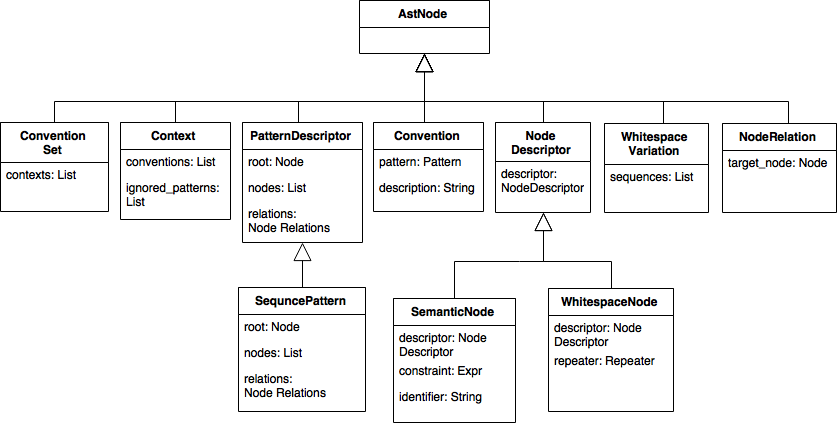
\includegraphics[width=\textwidth]{general}
\end{figure}


\begin{description}

\item\textbf{ConventionSet} represents a style guide. It comprises a number of conventions that form coherent guidelines. Attribute \texttt{contexts} is a list of Contexts that contain conventions.


\item\textbf{Context} represents a group of conventions that belong to the same semantic group (e.g. whitespacing, syntax preference, programming style). Attribute \texttt{conventions} is a list of Contexts that contain conventions. Attribute \texttt{ignored\_patterns} is a list of Patterns that are ignored while searching for the target pattern. For example, while searching for violations of semantic conventions, the whitespacing and indentation nodes are ignored.

\item\textbf{Convention} represents a rule that enforces specific constraints. Attribute \texttt{pattern} is the pattern that the convention targets. Attribute \texttt{description} is the description of the convention in natural text. This description is displayed to the user when a violation of the convention is discovered.

\item\textbf{PatternDescriptor} represents a description of a node or a combination of related nodes that given convention constraints. Attribute \texttt{root} is the top node described in the pattern. Attribute \texttt{nodes} is a collection of all nodes described by the pattern. Attribute \texttt{relations} is a collection of relationships between the nodes used in the pattern.

\item\textbf{NodeDescriptor} is an abstract class that contains a description of a Css Node. Attribute
\texttt{constraint} is an expression that designates constraints applied to the node.
Attribute \texttt{identifier} is a given string that can be used as a reference to the matched node.

\item\textbf{Node} represents a description of a node used in a PatternDescriptor. Attribute
\texttt{constraint} is an expression that designates constraints applied to the node.
Attribute \texttt{identifier} is a given string that can be used as a reference to the matched node.

\item\textbf{WhitespaceNode} represents a description of a whitespace node that references space,
newline, indentation symbols. Attribute \texttt{constraint} is an expression that designates
constraints applied to the node. Attribute \texttt{repeater} is an optional constraint that specific
the number of times a whitespace node can appear consecutively. Repeaters are useful to express
conventions that do not specify exact quantities of whitespace symbols. For example, the convention
``put at least one blank line between rules'' sets a lower limit of the number of blank lines, but
not an upper limit.

\item\textbf{NodeRelation} represents a relation between two Nodes. Attribute \texttt{target\_node}
designates a description of the Node targeted by the relation.

\end{description}


\begin{figure}[h!]
  \centering
  \caption{Abstract Syntax Expressions}
  \label{fig:expressions}
  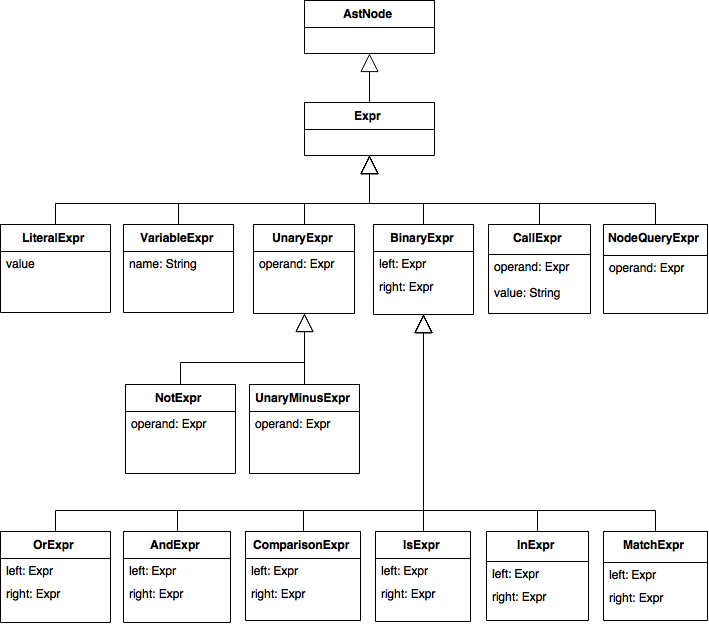
\includegraphics[width=\textwidth]{expr}
\end{figure}

A detailed view of the expressions in the abstract syntax of CssCoco is presented in Figure \ref{fig:expressions}. Following is a description of the subclasses of Expression:

\begin{description}

\item\textbf{LiteralExpr} represents an expression containing a literal value. Attribute \texttt{value} is the value of the literal expression.

\item\textbf{VariableExpr} represents a reference to a matched node. Attribute \texttt{name} is the identifier used to reference the node.

\item\textbf{UnaryExpr} represents expressions with a single operand. Attribute \texttt{operand} is operand of the expression.

\item\textbf{NotExpr} represents logical negation expression.

\item\textbf{UnaryMinusExpr} represents unary minus expression.

\item\textbf{BinaryExpr} represents expressions with a two operands.

Attributes \texttt{left} and \texttt{right} represent the first and second operands, respectively.

\item\textbf{OrExpr} represents logical disjunction expression.

\item\textbf{AndExpr} represents logical conjunction expression.

\item\textbf{ComparisonExpr} represents expression that compares two operands.

\item\textbf{IsExpr} represents expression that checks whether the first operand is of the given type, specified by the second operand.

\item\textbf{InExpr} represents expression that checks whether the first operand is present in a list of values, specified by the second operand.

\item\textbf{MatchExpr} represents expression that checks whether the first operand matches a regular expression, specified by the second operand.

\item\textbf{CallExpr} represents expression that invokes a API property or method of the operand. Attribute \texttt{operand} is the operand of the expression. Attribute \texttt{value} is the name of the API property or method that is invoked.

\item\textbf{NodeQueryExpr} represents expression that queries node context. Attribute \texttt{operand} is the node used as a reference point for the query.

\end{description}

\begin{figure}[h!]
  \centering
  \caption{Abstract Syntax Literal Expressions}
  \label{fig:literal}
  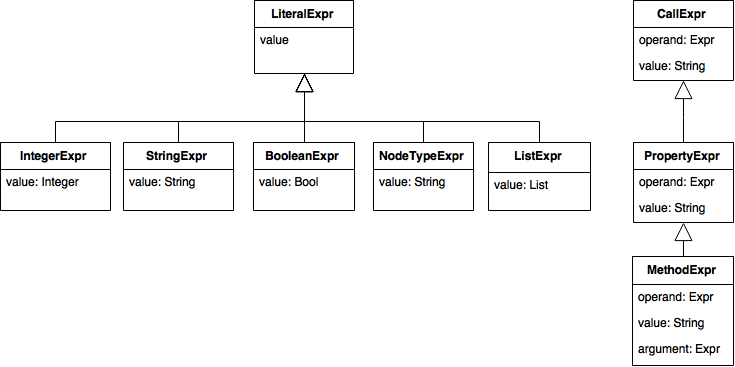
\includegraphics[width=0.9\textwidth]{literal}
\end{figure}

Figure \ref{fig:literal} presents a detailed view of the literal expressions used in the abstract syntax of CssCoco. Following is a listing of the classes. 

\begin{description}

\item\textbf{IntegerExpr} represents expression containing a integer value.

\item\textbf{DecimalExpr} represents expression containing a decimal value.

\item\textbf{StringExpr} represents expression containing a string value.

\item\textbf{BooleanExpr} represents expression containing a boolean value.

\item\textbf{ListExpr} represents expression containing a list value. The elements of the list are of type LiteralExpr.

\item\textbf{NodeTypeExpr} represents expression containing a string value that describes node type.

\end{description}

\begin{figure}[h!]
  \centering
  \caption{Abstract Syntax Literal Expressions}
  \label{fig:call}
  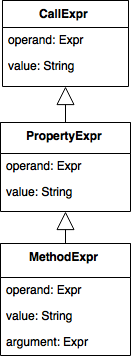
\includegraphics[width=0.2\textwidth]{call}
\end{figure}

Figure \ref{fig:call} presents a detailed view of the call expressions used in the abstract syntax of CssCoco. Following is a listing of the classes. 

\begin{description}

\item\textbf{PropertyExpr} represents an expression that returns the value of a property of the operand node. Attribute \texttt{operand} represents the node targeted by the expression. Attribute \texttt{value} holds the name of the property that is accessed.

\item\textbf{MethodExpr} represents an expression that returns invokes a method of the operand node. Attribute \texttt{argument} represents argument passed to the invoked method.

\end{description}

\begin{figure}[h!]
  \centering
  \caption{Abstract Syntax Node Query Expressions}
  \label{fig:nodequery}
  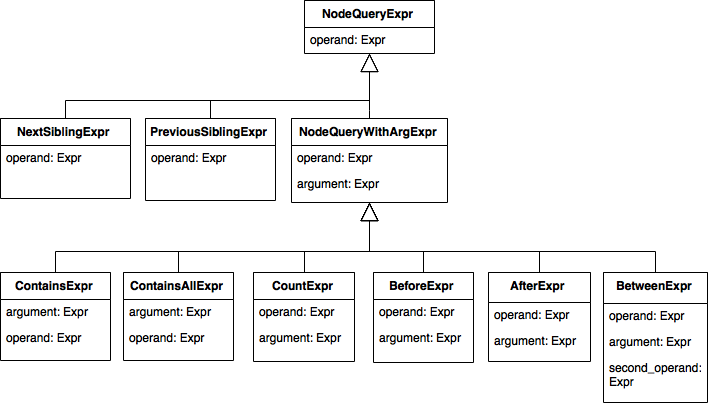
\includegraphics[width=0.9\textwidth]{nodequery}
\end{figure}

Figure \ref{fig:nodequery} presents an overview of the Node Query Expressions. The following listing describes the subclasses in details:

\begin{description}

\item\textbf{NextSiblingExpr} represents expression that returns the following sibling of the operand node.

\item\textbf{PreviousSiblingExpr} represents expression that returns the previous sibling of the operand node.

\item\textbf{NodeQueryWithArgExpr} represents expression that queries node context and uses additional constraints for the query. Attribute \texttt{argument} represents the additional constraints used by the query.

\item\textbf{ContainsExpr} represents an expression that checks whether the operand node contains a node that matches given constraints.

\item\textbf{ContainsAllExpr} represents an expression that checks whether the operand node contains nodes that match given constraints.

\item\textbf{CountExpr} represents an expression that counts the number of ancestor nodes of the operand that match a given constraint.

\item\textbf{BeforeExpr} represents an expression that checks whether a given whitespace variation appears before the operand node.

\item\textbf{AfterExpr} represents an expression that checks whether a given whitespace variation appears after the operand node.

\item\textbf{BetweenExpr} represents an expression that checks whether a given whitespace variation appears between the two operand nodes.

\end{description}

\subsection{Concrete syntax}

This section contains the concrete syntax of the designed DSL. Below are presented the grammar rules accompanied by the mapping to the abstract syntax of the language.


\begin{description}

\item\textbf{stylesheet} represents a style guide.

Abstract Syntax Mapping: ast.ConventionSet.

\begin{snippet}
\begin{verbatim}
stylesheet : context* ;
\end{verbatim}
\end{snippet}

\item\textbf{context} represents a group of logically related conventions. A single style guide can comprise a number of conventions that enforce various constraints, e.g. whitespacing, syntax preference, program style. Contexts group conventions that ignore the same nodes while searching for their violations.  

Abstract Syntax Mapping: ast.Context.

\begin{snippet}
\begin{verbatim}
context : Identifier ignore_clause? '{' convention* '}' ;
ignore_clause : 'ignore' (node_descriptor)+ (',' (node_descriptor)+)* ;
\end{verbatim}
\end{snippet}

\item\textbf{convention} represents a single rule in the style guide. Conventions are typically expressed by directly stating what is disallowed or describing a condition that if met, requires additional constraints. The former way of expressing conventions are represented by the \texttt{forbid} conventions. The latter approach uses the structure \texttt{find ... require ...}. To break down complex disallowing conventions, the structure \texttt{find ... forbid ...} has been introduced. This aims at improving readability of conventions. Additionally, the find conventions have a where clause which applies constraints for matching nodes. It is used to expression matching constraints that span over multiple nodes and therefore cannot be present in any of the node descriptors.

Abstract Syntax Mapping: ast.Convention.

\begin{snippet}
\begin{verbatim}
convention : 'forbid' pattern 'message' String
           | 'find' pattern ('where' logic_expr)? ('require'|'forbid') logic_expr 'message' String
           ;
\end{verbatim}
\end{snippet}

\item\textbf{pattern} represents a pattern of nodes and their relations. For example, it can describe a horizontal sequence of sibling nodes, a vertical pattern of nested nodes, or pairs of elements with a common parent. 

Abstract Syntax Mapping: ast.PatternDescriptor.

\begin{snippet}
\begin{verbatim}
pattern : node_declaration (('in'|'next-to') node_declaration)*
        | fork ('in' node_declaration)*
        ;
fork : '(' node_declaration (',' node_declaration)+ ')' ;
node_declaration : (Identifier '=')? semantic_node ;
\end{verbatim}
\end{snippet}

\item\textbf{node\_descriptor} represents a description of a node. It describes the type of the node and its additional constraints. 

Abstract Syntax Mapping: ast.NodeDescriptor.

\begin{snippet}
\begin{verbatim}
node_descriptor : node_type ('{' (logic_expr|repeater) '}')? ;
repeater : Integer ',' Integer? | (',')? Integer ;
\end{verbatim}
\end{snippet}


\item\textbf{logic\_expr} represents expressions that perform logic operations and glue arithmetic and type expressions. 

Abstract Syntax Mapping: ast.NotExpr, ast.AndExpr, ast.OrExpr and all arithmetic\_expression and type\_expression mappings.

\begin{snippet}
\begin{verbatim}
logic_expr : '(' logic_expr ')'
           | 'not' logic_expr
           | logic_expr 'and' logic_expr
           | logic_expr 'or' logic_expr
           | type_expr
           | arithmetic_expr
           ;
\end{verbatim}
\end{snippet}

\item\textbf{type\_expr} represents expressions that ensure node type and perform node queries on nodes. They are located in a separate parser rule because they interpret Identifiers as node type expressions instead of a API calls. 

Abstract Syntax Mapping: ast.IsExpr, ast.BeforeExpr, ast.AfterExpr, ast.BetweenExpr.

\begin{snippet}
\begin{verbatim}
type_expr : arithmetic_expr operator='is' Identifier
          | node_descriptor+ ('before' | 'after') type_operand
          | node_descriptor+ 'between' type_operand 'and' type_operand
          ;
type_operand : Identifier | semantic_node ;
\end{verbatim}
\end{snippet}

\item\textbf{arithmetic\_expr} represents arithmetic, comparison, set membership and regex expressions. These are located in a separate parser rule because they interpret identifiers as API calls instead of node type expressions.

Abstract Syntax Mapping: ast.UnaryMinus, ast.UnaryPlus, ast.LessThan, ast.LessThanOrEq, ast.GreaterThan, ast.GreaterThanOrEq, ast.Equal, ast.NotEqual, ast.InExpr, ast.MatchExpr, ast.LiteralExpr.

\begin{snippet}
\begin{verbatim}
arithmetic_expr : ('-'|'+') arithmetic_expr
                | arithmetic_expr ('<'|'>'|'<='|'>='|'=='|'!=') arithmetic_expr
                | arithmetic_expr ('in'|'not in'|'match'|'not match') arithmetic_expr
                | call_expression
                | element
                ;
element : Boolean | Decimal | Integer | String | list_ ;
\end{verbatim}
\end{snippet}

\item\textbf{call\_expression} represents an API call expression and also node query expression.

Abstract Syntax Mapping: ast.CallExpr and ast.NodeQueryExpr.

\begin{snippet}
\begin{verbatim}
call_expression : call_expression '.' call_expression
                | Identifier ('(' (element | semantic_node ) ')')? 
                ;
\end{verbatim}
\end{snippet}

\item\textbf{Boolean:} represents Boolean literal expression. 

Abstract Syntax Mapping: ast.BooleanExpr.

\begin{snippet}
\begin{verbatim}
Boolean : 'true' | 'True' | 'false' | 'False' ;
\end{verbatim}
\end{snippet}

\item\textbf{String:} represents String literal expression.

Abstract Syntax Mapping: ast.StringExpr.

\begin{snippet}
\begin{verbatim}
String : "'" (EscapeSequence | ~['])*? "'" ;
EscapeSequence : "\\" "'" ;
\end{verbatim}
\end{snippet}

\item\textbf{Integer:} represents Integer literal expression. 

Abstract Syntax Mapping: ast.IntegerExpr.

\begin{snippet}
\begin{verbatim}
Integer : (ZeroDigit | NonZeroDigit Digit*) ;
Digit : ZeroDigit | NonZeroDigit ;
NonZeroDigit : [1-9] ;
ZeroDigit : [0] ;
\end{verbatim}
\end{snippet}

\item\textbf{Decimal:} represents Decimal literal expression. 

Abstract Syntax Mapping: ast.DecimalExpr.

\begin{snippet}
\begin{verbatim}
Decimal : ( NonZeroDigit Digit* | ZeroDigit? ) '.' Digit+ ;
Digit : ZeroDigit | NonZeroDigit ;
NonZeroDigit : [1-9] ;
ZeroDigit : [0] ;
\end{verbatim}
\end{snippet}

\item\textbf{list} and \textbf{list\_element} represent the List literal expression. 

Abstract Syntax Mapping: ast.ListExpr.

\begin{snippet}
\begin{verbatim}
list_ : '[' list_element (',' list_element)* ']' ;
list_element : Integer | Decimal | String | semantic_node ;
Letter : [a-zA-Z] ;
Identifier : (Letter)(Letter|Digit|'_'|'-')* ;
\end{verbatim}
\end{snippet}

\item\textbf{type\_expression} represents the NodeType literal expression.

Abstract Syntax Mapping: ast.NodeType.

\begin{snippet}
\begin{verbatim}
node_type : '(' node_type ')'
          | 'not' node_type
          | node_type 'and' node_type
          | node_type 'or' node_type
          | Identifier
          ;
\end{verbatim}
\end{snippet}

\end{description}

\subsection{Prototype}

An prototype of CssCoco is implemented and publicly available. Currently, the prototype consists of
two parts: a standalone python 3 package and a plug-in for Sublime Text editor. The source code of
both parts is publicly available at \url{https://github.com/boryanagoncharenko/CssCoco} and at
\url{https://github.com/boryanagoncharenko/Sublime-CssCoco}, respectively.

\section{Validation}

The method chosen for validating the designed domain-specific language is ontological analysis,
since it is a widely accepted way for evaluating software notations~\cite{opdahl2002ontological}~\cite{green2000integrated}~\cite{moody2009physics}~\cite{parsons1997using}~\cite{weber1996analytical}.
The particular approach used for conducting ontological analysis consists of several steps. First, a
domain-specific ontology is designed. Second, the ontology is used as a reference point for the
interpretation and representation mappings. Third, emerged anomalies are analyzed and conclusion
about the quality of the notation is made.

\subsection{Ontology design}

The first stage of validation requires designing a domain-specific ontology. The specific domain of
the developed ontology is limited to detecting violations of CSS code conventions. In other words,
the designed ontology tries to capture only the concepts and their relations, that exist when an
agent searches a CSS program for violations of given set of code conventions.

The designed domain-specific ontology is based on the BWW top-level
ontology~\cite{wand1990ontological}, i.e. it uses the high-level categories of the BWW ontology to
describe the objects, concepts and entities in the specific domain. The rationale behind the
decision to use BWW ontology is that it has been the leading ontology used for ontological
analysis~\cite{moody2009physics}. The main ontological constructs used in the BWW ontology are
listed in section 2.1.

The designed ontology is presented using several approaches. As recommended by Wand and Weber, the
ontology is presented using a dictionary comprising definitions of entities in natural text and,
second, using Backus-Naur Form (BNF) notation~\cite{wand1995deep}~\cite{rosemann2002developing}.
Additionally, a system diagram is included to provide a better view of the couplings between the
different entities. The ontology is intentionally not presented using Unified Modeling Language or
Entity-Relationship diagrams. These modeling languages are subjects of ontological analysis
themselves and therefore are not suitable for expressing an ontology.

Following is a list with the main concepts discovered in the domain along with their descriptions.
The used BWW concepts are written in \textit{italics} and the domain-specific concepts are written
in \textbf{bold}.

\begin{description}

\item\textit{Class} \textbf{Style Guide} describes the coding practices adopted in the context of a single project, organization, community or language. An individual Style Guide is a \textit{composite thing} built of Conventions and their relations. Conventions in a Style Guide are interpreted together to form a coherent set of guidelines.

\textit{Property} \textbf{Conventions} refers to the conventions contained in the Style Guide.


\item\textit{Class} \textbf{Convention} is a specific rule that imposes constraints on the CSS program. It is the building block of Style Guides. An individual Convention is a \textit{composite thing} that contains a Context.

\textit{Intrinsic Property} \textbf{Description} contains the reasoning behind the Convention.

\textit{Hereditary Property} \textbf{Ignored Constructs} denotes the description of constructs that should be ignored while searching for the Convention's Context. It is inherited by the Context thing that builds a Convention.


\item\textit{Class} \textbf{Context} is a description of a Pattern that the Convention forbids. An individual Context is a \textit{composite thing} that comprises a number of logically related Constraints. When a Pattern in the current Stylesheet fulfills all Constraints in the Context, a Violation is discovered.

\textit{Property} \textbf{Ignored Constructs} are descriptions of Patterns that need to be disregarded while searching for the current Context. In fact, the property denotes a collection of Contexts.


\item\textit{Class} \textbf{Constraint} is a specific restriction that needs to be fulfilled. They
are used in a \textbf{Context} to build a description of a \textbf{Pattern}. Constraints are
individual requirements that are imposed on subjects. Based on the value of the requirement, there
are different types of Constraints represented below as \textit{subclasses}.

\textit{Property} \textbf{Subject} indicates the thing is being constrained.

\textit{Property} \textbf{Requirement} denotes the particular limitation applied to the Subject.


\item\textit{Subclass} \textbf{Existence Constraint} is a type of Constraint that requires existence of the subject. 

\textit{Property} \textbf{Subject} indicates the thing is being constrained.

\textit{Property} \textbf{Requirement} denotes the particular limitation applied to the Subject. Specifically, that the Subject must exist.


\item\textit{Subclass} \textbf{Comparison Constraint} is a type of Constraint that compares the subject to another value.

\textit{Property} \textbf{Subject} indicates the thing is being constrained.

\textit{Property} \textbf{Requirement} denotes the particular limitation applied to the Subject. Specifically, that the Subject must be related to the Value in a given way.

\textit{Property} \textbf{Value} denotes the value that is used for the comparison.


\item\textit{Subclass} \textbf{Type Constraint} is a type of Constraint that checks whether the subject is of a given type.

\textit{Property} \textbf{Subject} indicates the thing is being constrained.

\textit{Property} \textbf{Requirement} denotes the particular limitation applied to the Subject. Specifically, that the Subject must be of the given type.

\textit{Property} \textbf{Value} denotes the type that the subject should meet to satisfy the constraint.


\item\textit{Subclass} \textbf{Textual Form Constraint} is a type of Constraint that imposes restrictions on the textual representation of the subject.

\textit{Property} \textbf{Subject} indicates the thing is being constrained.

\textit{Property} \textbf{Requirement} denotes the particular limitation applied to the Subject. Specifically, that the Subject must be equal to the given Value.

\textit{Property} \textbf{Value} denotes the textual form that the Subject should meet for the constraint to be satisfied.


\item\textit{Subclass} \textbf{Set Membership Constraint} is a type of Constraint that requires the subject to be a member of a set.

\textit{Property} \textbf{Subject} indicates the thing is being constrained.

\textit{Property} \textbf{Requirement} denotes the particular limitation applied to the Subject. Specifically, that the Subject must be a member of the Value.

\textit{Property} \textbf{Value} denotes the set that the subject should be present at for the constraint to be satisfied.


\item\textit{Class} \textbf{Literal Value} is a thing that represents a constant value. It includes numbers, strings, boolean values etc.

\textit{Property} \textbf{Value} denotes the specific value possessed by the literal.


\item\textit{Class} \textbf{Violation Log} is the final product of a violations search. An individual Violation Log is a composite thing that contains Violations.

\textit{Property} \textbf{Number of Violations} indicates the size of the Violation Log. 


\item\textit{Class} \textbf{Violation} A Violation occurs when a Pattern that matches the Context of a Convention is found.

\textit{Property} \textbf{Description} explains in natural text what causes the Violation. Typically, the Description is extracted from the Convention that the Violation breaks.

\textit{Property} \textbf{Position in Stylesheet} indicates the location of the Pattern that violates the Convention in the Stylesheet. 


\item\textit{Class} \textbf{Stylesheet} is the CSS code that needs to be checked for compliance with the Style Guide. An instance of Stylesheet is a composite thing that comprises a number of Constructs.

\textit{Property} \textbf{Checked} indicates whether a Stylesheet has been checked for compliance to a given Style Guide. 


\item\textit{Class} \textbf{Construct} is a part of the Stylesheet. It can refer to nodes in the CSS abstract syntax tree, concrete syntax tree and parse tree. Examples include whitespacing, indentation, comments, colons, delimiters, rulesets, declarations, etc.

\textit{Property} \textbf{Property} encapsulates properties of nodes specific to the CSS domain. For example, the type and the string representation of the node are its properties. Similarly, specific CSS Nodes can expose properties that are tightly coupled to the CSS domain, such as release date or vendor name of a CSS property.


\item\textit{Class} \textbf{Pattern} is a particular part of the CSS program that matches the description of a Context. An instance of a Pattern is a composite thing built from one or many Constructs and Relations between them.

\textit{Property} \textbf{Constructs} denotes the constructs that are contained in the Pattern.


\item\textit{Event} \textbf{Search for Violations in Stylesheet} occurs when the developer completes the search for violations in a Stylesheet, a Violation Log is created and the state. When the search is completed, the Stylesheet is considered checked for compliance to the Style Guide.

\textit{New State} \textbf{Violation Log} \{ Violations = value \}

\textit{New State} \textbf{Stylesheet} \{ Checked = True \}


\item\textit{Event} \textbf{Context (Convention) Discovered} occurs when the Context of a convention is discovered, a Violation is recorded in the Violation Log. The state of the Violation contain its description and position in Stylesheet.

\textit{New State} \textbf{Violation} \{ Description = value, Position in Stylesheet = value \}


\item\textit{Event} \textbf{Stylesheet modified} occurs when the Constructs in the Stylesheet are modified. The state of the Stylesheet is changed to unchecked for compliance.

\textit{New State} \textbf{Stylesheet} \{ Checked = False \}


\item\textit{Event} \textbf{Style Guide modified} occurs when any of the parts of a Style Guide are modified. This event changes the state of the Stylesheet to unchecked for compliance.

\textit{New State} \textbf{Stylesheet} \{ Checked = False \}

\end{description}


Most of the definitions in the ontology refer to simple concepts that appear in the code conventions
domain. For example the concept of a Style Guide refers to a collection of coherent conventions. A
Style Guide on its own does not have any emergent or intrinsic properties and, thus, it is defined
through the conventions it comprises. Note that in reality a Style Guide may contain a number of
intrinsic properties, for example a Style Guide may have an author and contributors. Such
properties, however, are not considered part of the specific domain, and thus lie outside the scope
of the ontology.

A Convention is defined as the building block of a Style Guide. However, the ontological concept of
a Convention is slightly different than what is used as a convention in the domain analysis section.
For example, domain analysis indicates that there are two types of conventions: forbid and require.
The former type of conventions describes directly their violations. The latter type describes a
pattern that, when found, additional requirements must be met and in case they are not met, a
violation is discovered. For example, the violation \textit{Do not use id selectors} tells that id
selectors are violations. The convention \textit{Strings should be with single quotes} states that
strings must have single quotes, and a violation is discovered if the found string does not.
Convention types are not related to the meaning of conventions but to the way they are expressed. A
convention with the same meaning could be expressed using both structures: \textit{Strings should be
with single quotes} and \textit{Forbid strings with double quotes}. Since ontological concepts are
concerned with the meaning of things and have to be independent of the language used to express
them, the ontology does not possess subclasses of Convention.

A Context is a description of things that are disallowed by a Convention, i.e. it states explicitly
what Patterns violate a Convention. In this sense, the meaning of a Convention is always expressed
through the possible violations of that Convention. A Context is built from a number of Constraints.
While a Context aims at describing a whole violation pattern, a Constraint refers to a single
specific requirement. A Constraint always has a subject and a requirement. The subject is the object
that is being constraint and the requirement refers to the specific limitation that is applied to
the subject. Based on the value of the requirement property, there are different types of
Constraints. For example, a Comparison Constraint requires the subject to be equal or greater than a
given value and the Type Constraint require the subject to be of a particular type. The Existence
Constraint requires the subject to exist.

Since Conventions are used to constraint CSS code, subjects are typically Constructs or their
properties. A Construct denotes a concrete part of the Stylesheet, e.g. newline, semicolon,
declaration, ruleset etc. Each Construct exposes a number of properties that are tightly coupled to
the function of the Construct in the stylesheet. For example, a property construct has properties
that indicate whether it is vendor-specific and its release date.

Patterns are composed of Constructs. The Constructs in the Pattern do not need to form a coherent
valid Stylesheet and they do not have to be adjacent or directly related. In fact, they could be
scattered across the whole Stylesheet. Patterns denote the concrete Constructs that match the
description provided by the Context of a Convention. In this sense, they are the specific instances
of Violations.

Definitions of the ontological concepts in the listing above often state that an instance of a
class is a composite thing that consists of other things. To provide a better understanding of the
way composite things are constructed, the same concepts are also expressed using BNF notation:

\begin{snippet}
\begin{verbatim}
STYLE_GUIDE     ::= CONVENTIONS
CONVENTIONS     ::= CONVENTIONS CONVENTION | CONVENTION 
CONVETION       ::= CONTEXT
CONTEXT         ::= CONSTRAINTS
CONSTRAINTS     ::= CONSTRAINTS CONSTRAINT | CONSTRAINT
CONSTRAINT      ::= EXISTENCE_CONSTRAINT | COMPARISON_CONSTRAINT | TYPE_CONSTRAINT  
                  | TEXT_CONSTRAINT | SET_CONSTRAINT
VIOLATION_LOG   ::= VIOLATIONS
VIOLATIONS      ::= VIOLATIONS VIOLATION | VIOLATION | EPSILON
STYLESHEET      ::= CONSTRUCTS
CONSTRUCTS      ::= CONSTRUCTS CONSTRUCT | CONSTRUCT
PATTERN         ::= CONSTRUCTS
\end{verbatim}
\end{snippet}

The grammar above illustrates that a Style Guide needs to contain one or more Conventions.
Similarly, a Context requires at least one Constraint in order to exist. A Violation Log, however,
could exist without any Violations in the cases when a Stylesheet is checked for conformance to a
Style Guide and no violations are discovered. Both Stylesheet and Pattern are defined through 1 or
more Constructs. Note that the concept of Stylesheet does not map to a CSS file, but to the whole
CSS code that needs to be processed, regardless of type of CSS. This is why a Stylesheet requires at
least one Construct in order to exist.

While the above grammar presents the composition of things, it does not illustrate how things
interact with each other. To provide a better understanding of the dynamics between things defined
in the ontology, a graph of the system is presented in Figure \ref{fig:couplings}.

\begin{figure}[h!]
  \centering
  \caption{Graph of the system}
  \label{fig:couplings}
  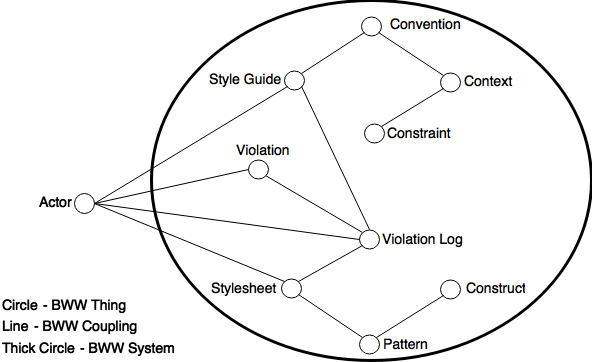
\includegraphics[width=0.8\textwidth]{couplings}
\end{figure}

According to the theory, a coupling occurs when the existence of a given thing affects the history
of another thing and, in turn, history is defined as the chronological ordered states that a thing
traverses~\cite{wand1990ontological}. Thus, in the domain-specific ontology a coupling exists
between the Style Guide and the Convention things, because the existence of a Convention alters the
state of the Style Guide. Similarly, a Context changes the state of a Convention and a Constraint
affects the state of a Context.

There are also couplings between Construct, Pattern and Stylesheet things. Both Stylesheet and
Pattern are composed of Constructs, and thus affected by their existence. Since a Pattern is a
specific occurrence of a combination of Constructs, it is also coupled to Stylesheet.

A Violation is coupled to a Violation Log, since the presence of a new a Violation alters the state
of the log. Further, a Violation Log contains information about the violations of a particular Style
Guide that occur in a specific Stylesheet. In this sense, a Violation Log is a function of a Style
Guide and a Stylesheet and it is coupled to both things.

There are a number of external events that can change the state of the system. An actor can initiate
search for violations, which affects the state of the Violation Log and the Stylesheet. If during
the search an actor discovers a violation, the state of the Violation is altered. Also, an actor can
modify the Stylesheet and the Style Guide. Thus, couplings exist between the Actor and the
Stylesheet, Violation, Violation Log and Style Guide.

\subsection{Ontological analysis}

The ontological analysis draws comparison between the designed domain-specific ontology and the
domain-specific language. It consists of two mappings: representation and interpretation. The former
mapping matches the ontology to the language and the latter - the language to the ontology.
Typically ontological analysis is used to compare the abstract syntax of the language constructs to
the concepts of an ontology. However, the designed ontology contains concepts that fall outside the
scope of the abstract syntax. For example, the notion of Violation Log has a corresponding class in
the system. However, that class denotes the product of the violations search and is not part of the
abstract syntax. The particular approach chosen to conduct ontological analysis is to compare the
abstract syntax of the language to the ontology. Additionally, all remaining ontological constructs
are mapped to their representation in the whole system. For example, the ontological concept of a
Violation Log is matched with the Violation Log class in the analysis module.

\subsubsection{Representation and Interpretation Mappings} 

This subsection contains the two mappings between the modeling grammar and domain-specific ontology.
Table \ref{tab:representation} presents the representation mapping. The left-hand side of the table
contains the ontological constructs in the order of definition and the right-hand side comprises the
corresponding modeling grammar construct. Table \ref{tab:interpretation} presents the interpretation
mapping. The left-hand side contains classes from the abstract syntax, followed by classes that have
a representation in the ontology and the right-hand side contains the corresponding ontological
construct.

\begin{table}[t]
\begin{center}
\begin{longtable}{ | p{20em} | p{20em} | } 
\hline
 &  \\
Ontological constructs & Grammar constructs \\
 &  \\
\hline
Style Guide & Convention Set \\ \hline
Conventions (Style Guide) & Contexts (Convention Set), Conventions (Context) \\ \hline
Convention & Convention \\ \hline
Description (Convention) & Description (Convention) \\ \hline
Context & Pattern Descriptor \\ \hline
Ignored Constructs (Context) &  Context \\ \hline

Constraint & Comparison, Is, In, Match, Node Query, Not, And, Or Expressions \\ \hline
Subject (Constraint) & Operand of Expression \\ \hline
Requirement (Constraint) & Subclasses of Expression \\ \hline
Value (Constraint Subclasses) & Second Operand of Binary Expression \\ \hline
Existence Constraint & Node Descriptor, Node Relation, Node Query Expression \\ \hline
Comparison Constraint & Comparison Expression \\ \hline
Type Constraint & Is Expression \\ \hline
Textual Form Constraint & Match Expression \\ \hline
Set Membership Constraint & In Expression \\ \hline
Literal Value & Literal Expression \\ \hline
Value (Literal Value) & Value (Literal Expression) \\ \hline

Violation Log & Violation Log \\ \hline
Violations (Violation Log) & Violations (Violation Log) \\ \hline
Violation & Violation \\ \hline
Description (Violation) & Description (Violation) \\ \hline
Position in Stylesheet (Violation) & Position (Violation) \\ \hline

Stylesheet & Stylesheet Node \\ \hline
Checked (Stylesheet) & - \\ \hline
Construct & Variable Expression \\ \hline
Property (Construct) & Call Expression \\ \hline
Pattern & Css Pattern \\ \hline
Constructs (Pattern) & Nodes (Css Pattern) \\ \hline
\end{longtable}
\end{center}
\caption{
	\label{tab:representation}
	Representation mapping}
\end{table}


\begin{center}
\begin{longtable}{ | p{20em} | p{20em} | } 
\caption{Interpretation mapping}
\label{tab:interpretation}\\
\hline
 &  \\
Grammar constructs & Ontological constructs  \\
 &  \\
\hline

Convention Set & Style Guide \\ \hline
Contexts (Convention Set) & partly Conventions (Style Guide) \\ \hline
Context & Ignored Constructs (Context) \\ \hline
Conventions (Context) & partly Conventions (Style Guide) \\ \hline
Convention & Convention \\ \hline
Description property (Convention) & Description (Convention) \\ \hline
Pattern Descriptor & Context \\ \hline
Node Descriptor & partly Existence Constraint \\ \hline
Node Relation & partly Existence Constraint \\ \hline

Literal Expression & Literal Value \\ \hline
Variable Expression & Construct \\ \hline
Not Expression & partly Constraint \\ \hline
And Expression & partly Constraint \\ \hline
Or Expression & partly Constraint \\ \hline
Comparison Expression & Comparison Constraint \\ \hline
Match Expression & Textual Form Constraint \\ \hline
In Expression & Set Membership Constraint \\ \hline
Is Expression & Type Constraint \\ \hline
Call Expression & Property (Construct) \\ \hline
Node Query Expression & partly Existence Constraint \\ \hline

Css Pattern & Pattern \\ \hline
Nodes (Css Pattern) & Constructs (Pattern) \\ \hline
StylesheetNode & Stylesheet \\ \hline
Violations Log & Violations Log \\ \hline
Violations (Violations Log) & Violations (Violation Log) \\ \hline
Violation & Violation \\ \hline
Description (Violation) & Description (Violation) \\ \hline
Position (Violation) & Position in Stylesheet (Violation) \\ \hline
\end{longtable}
\end{center}


\textbf{Ontological Classes and Subclasses}

The ontological concept of Style Guide is represented in the modeling grammar as a Convention Set.
Similarly, the notion of Convention maps to the Convention class and the concept of Context maps to
the Pattern Descriptor class.

The ontological concept of Constraint appears in the modeling grammar as a number of Expressions.
These include Expressions used in mappings for the subclasses of Constraint: Comparison Expression,
Is Expression, Match Expression, In Expression and Node Query Expression. Additionally, the
Constraint is mapped to And, Not and Or Expressions. These constructs cannot serve as Constraints
themselves but are used to form more complex Constraints.

The mappings for most of the Constraint subclasses are straight forward. For example, the Comparison
Constraint is represented as a Comparison Expression and the Type Constraint appears as an Is
Expression. Similarly, the Textual Form Constraint is a Match Expression and the Set Membership
Constraint maps to the In Expression. That said, the Existence Constraint require further attention.
As defined in the ontology, the Existence Constraint requires the subject to exist. In the modeling
grammar this concept is indirectly presented using multiple structures. Nodes in a pattern are
specified using two ways: either through using Node Descriptor and Node Relations, or through Node
Query Expression. The modeling grammar describes the anchor nodes from the pattern and their parent
nodes using the former approach and nodes that are nested in the anchor nodes using the latter. For
example, when a the pattern that needs to be matched is a ruleset that contains a z-index property
and appears in a media query, the existence of the media query and the ruleset (and their
relationship) is described using Node Descriptors and a Node Relation. The existence of the property
contained in the ruleset is denoted using a Node Query Expression.

The ontological constructs of Violation Log and Violation are mapped to the Violation Log and
Violation classes, respectively. The notion of a Stylesheet is represented by the Stylesheet Node in
the solution and a Pattern is mapped to Css Pattern. The concept of a Construct is represented in
the abstract syntax tree as a Variable Expression. The reason behind this mapping is that in the
modeling grammar Variable Expression denote only Constructs.

\textbf{Ontological Properties}

The majority of the ontological properties are mapped to a single construct in the solution. For
example, the Description property of Convention class in the ontology is directly mapped to the
Description property of the Convention class in the modeling grammar. However, some of the property
mappings are not that obvious. For example, the ontological property Conventions of class Style
Guide is represented by a combination of properties in the solution: Contexts of Convention Set and
Conventions of Context. Also, the notion of Ignored Constructs maps to the Context class in the
solution. The reason for these mappings comes from the fact that the solution groups together
conventions with identical ignored constructs. As stated in the ontology description, each
convention specifies a set of constructs that need to be ignored while searching for its violations.
For example, while evaluating the constraints of conventions related to newlines, the indentation
constructs are typically ignored. Because the ignored constructs are similar for most of the
conventions, the modeling grammar groups conventions that use the same ignored constructs into
contexts. Thus, the Convention Set contains Contexts and a Context specifies the ignored constructs
of all convention that it contains.

The Subject and the Value of a Constraint are mapped to the operands of Expression. The subclasses
of Constraint are based on the different values of the Requirement property. Similarly, the
Requirement of Constraint is expressed through child classes of Expression.

The ontological property Violations of the Violation Log construct appears in the modeling grammar
as property Violations of the Violation Log class. The Violation class exposes Description and
Position properties that map to the ontological properties Description and Position in Stylesheet.
The Checked property of Stylesheet does not have a representation in the system. The property
Property of Construct is denoted in the abstract syntax using a Call Expression.

\subsection{Ontological Evaluation of the System}

The primary purpose of the representation and interpretation mappings between the ontology and the
modeling grammar is discovering discrepancies between the two entities. The four types of
ontological anomalies are considered in the following subsections.

\subsubsection{Redundant Constructs} 

Construct redundancy is a type of anomaly in which more than one modeling construct can represent a
single ontological construct. The representation mapping illustrates that there are three candidates
for this discrepancy. 

First, the Conventions property of Style Guide is matched to Contexts property of Convention Set and
the Conventions property of Context. Such mapping is required since the modeling grammar groups
Conventions that share the same Ignored Constructs in a Context. Thus, a Style Guide in the modeling
grammar does not possess conventions but a number of Contexts that, in turn, contain conventions. In
this sense, the properties Contexts and Conventions together represent the concept of Conventions.

Note that redundancy occurs when the two grammar constructs can independently represent the same
ontological concept. In the specific case, however, none of the constructs taken individually can
express the property. It is their combination that represents the concept. Mapping a single
ontological concept to a combination of modeling grammar constructs is an accepted approach and has
been done in multiple studies~\cite{gehlert2007toward}. Thus, the two constructs are not
considered redundant.

Second, the Comparison, Is, In, Match, Node Query, And, Or and Not Expressions map to the concept of
Constraint. As defined in the ontology, a Constraint is a class that has multiple subclasses
depending on the specific requirement they enforce. In this sense, Expressions that map to any
subclasses of Constraint, also map the Constraint class. These are the Comparison, Is, In, Match and
Node Query Expressions. The remaining part of Expressions are And, Or and Not. These Expressions are
used to combine Constraints into complex Constraints. For example, a Context may contain a number of
Constraints that need to be put together using the And Expression. However, the And Expression
itself cannot be a Constraint - it is used to build Constraints. In this sense, none of the three
Expressions can independently represent a Constraint. Their combination with the Expressions mapped
to the subclasses of Constraint expresses the concept of Constraint. Thus, the expressions are not
considered redundant.

Third, the Existence Constraint is mapped to the Node Descriptor, Node Relation and Node Query
Expressions. Existence Constraint is a type of Constraint that requires the Subject to exist. For
example, the convention \textit{Use a fallback property for RGBA and HSLA values} requires the
fallback declaration to have the same property as the matched declaration and the value of the
fallback declaration to be different than RGBA or HSLA. However, before these, the convention
requires the fallback declaration to exist.

In the modeling grammar, when a Pattern Descriptor refers to multiple nodes, the presence of a Node
Descriptor denotes the existence of CSS Node and the Node Relation specifies how the Nodes are
connected in the Pattern Descriptor. As described in the domain analysis section, each Pattern
Descriptor has one of more anchors. These are the specific nodes that need to be iterated. While the
Node Descriptors and Node Relations describe the anchor nodes in the Pattern and their parent nodes,
the Node Query Expression is used to describe parts of the pattern that are nested in the anchors.

As with the previous two cases, the ontological concept cannot be represented by Node Descriptors
and Node Relations or by Node Query Expressions taken individually. Their combined use allows
expressing patterns. For this reason, the constructs are not considered redundant.


\subsubsection{Construct Overload}

Construct overload emerges when a single modeling construct can represent a number of ontological
constructs. In the interpretation and representation mappings every language construct is assigned a
single ontological construct. In this sense, there are not candidates for overload discrepancy.

\subsubsection{Construct Excess}

Construct excess is a discrepancy in which a modeling construct does not have a mapping to an
ontological construct. Typically, ontological analysis is performed through comparing the abstract
syntax of the domain-specific language to the ontology. In the interpretation mapping all constructs
that belong to the abstract syntax are mapped to an ontological construct. Thus, there are not
candidates for construct excess from the abstract syntax.

\subsubsection{Construct Deficit}

Construct deficit appears when an ontological construct does not have a corresponding modeling
structure. A candidate for such discrepancy is the property Checked of class Stylesheet as it
appears without a matching construct in the system. However, maintaining the status of a Stylesheet
is considered outside the scope of the system. Such functionality is highly dependent on the
specific information offered by the IDE or text editor. Support for this property remains in the
environment of the system. In this sense, the candidate is not considered an occurrence of deficit.


\subsubsection{Results}

In this section are presented the interpretation and representation mappings between the modeling
grammar and the designed domain-specific ontology. Further, all types of discrepancies are analyzed
and argumentation is provided why they should not be considered anomalies. Having the analysis in
mind, it can be concluded that the ontological analysis provides sufficient evidence to consider the
designed system both ontologically clear and complete.

%%%%%%%%%%%%%%%%%%%%%%%%%%%%%%%%%%%%%%%%%%%%%%%%%%%%%%%%%%%%%%%%%%%%%%%%%%%%%%%

\chapter{Conclusion}
\label{sec:conclusion}

The variability of CSS conventions used in practice cannot be handled by existing tools. Thus, developers often need to make sure their code complies to a given style guide manually. The thesis offers a solution to this problem. The contribution of this thesis is threefold. First, the need for CSS conventions is evaluated and
evidence that CSS is still handcrafted is provided. Second, a list of the existing code conventions
and their analysis is presented. Third, a domain-specific language that is capable of expressing the
gathered conventions is proposed. A prototype of language and its interpreter are implemented to
enable automatic detection of violations.

{%\tiny
\bibliographystyle{ieeetr}
\bibliography{thesis}
}

\end{document}
